\documentclass[fleqn,10pt,lineno]{wlpeerj}\usepackage[]{graphicx}\usepackage[]{color}
%% maxwidth is the original width if it is less than linewidth
%% otherwise use linewidth (to make sure the graphics do not exceed the margin)
\makeatletter
\def\maxwidth{ %
  \ifdim\Gin@nat@width>\linewidth
    \linewidth
  \else
    \Gin@nat@width
  \fi
}
\makeatother

\definecolor{fgcolor}{rgb}{0.345, 0.345, 0.345}
\newcommand{\hlnum}[1]{\textcolor[rgb]{0.686,0.059,0.569}{#1}}%
\newcommand{\hlstr}[1]{\textcolor[rgb]{0.192,0.494,0.8}{#1}}%
\newcommand{\hlcom}[1]{\textcolor[rgb]{0.678,0.584,0.686}{\textit{#1}}}%
\newcommand{\hlopt}[1]{\textcolor[rgb]{0,0,0}{#1}}%
\newcommand{\hlstd}[1]{\textcolor[rgb]{0.345,0.345,0.345}{#1}}%
\newcommand{\hlkwa}[1]{\textcolor[rgb]{0.161,0.373,0.58}{\textbf{#1}}}%
\newcommand{\hlkwb}[1]{\textcolor[rgb]{0.69,0.353,0.396}{#1}}%
\newcommand{\hlkwc}[1]{\textcolor[rgb]{0.333,0.667,0.333}{#1}}%
\newcommand{\hlkwd}[1]{\textcolor[rgb]{0.737,0.353,0.396}{\textbf{#1}}}%
\let\hlipl\hlkwb

\usepackage{framed}
\makeatletter
\newenvironment{kframe}{%
 \def\at@end@of@kframe{}%
 \ifinner\ifhmode%
  \def\at@end@of@kframe{\end{minipage}}%
  \begin{minipage}{\columnwidth}%
 \fi\fi%
 \def\FrameCommand##1{\hskip\@totalleftmargin \hskip-\fboxsep
 \colorbox{shadecolor}{##1}\hskip-\fboxsep
     % There is no \\@totalrightmargin, so:
     \hskip-\linewidth \hskip-\@totalleftmargin \hskip\columnwidth}%
 \MakeFramed {\advance\hsize-\width
   \@totalleftmargin\z@ \linewidth\hsize
   \@setminipage}}%
 {\par\unskip\endMakeFramed%
 \at@end@of@kframe}
\makeatother

\definecolor{shadecolor}{rgb}{.97, .97, .97}
\definecolor{messagecolor}{rgb}{0, 0, 0}
\definecolor{warningcolor}{rgb}{1, 0, 1}
\definecolor{errorcolor}{rgb}{1, 0, 0}
\newenvironment{knitrout}{}{} % an empty environment to be redefined in TeX

\usepackage{alltt} % for journal submissions
\usepackage{hyperref} % \documentclass[fleqn,10pt]{wlpeerj} % for preprint submissions

\title{Using metagenomic methods to detect organismal contaminants in microbial materials.}

\author[1]{Nathan D. Olson}
\author[1]{Justin M. Zook}
\author[1]{Jayne B. Morrow}
\author[1]{Nancy J. Lin}
\affil[1]{Material Measurement Laboratory, National Institute of Standards and Technology}

\keywords{Genomic Purity, Whole Genome Sequencing, Bioinformatics, Biodetection, Microbial Material, Reference Material}

\begin{abstract}
High sensitivity methods such as next generation sequencing and polymerase chain reaction (PCR) are adversely impacted by organismal and DNA contaminants.
Current methods for detecting contaminants in microbial materials (genomic DNA and cultures) are not sensitive enough and require either a known or culturable contaminant.
Therefore, high sensitivity methods not requiring \textit{a priori} assumptions about the contaminant are needed.
We demonstrate the use of whole genome sequencing (WGS) and a metagenomic taxonomic classification algorithm for assessing the organismal purity of a microbial material.
Using this proposed method we characterized the types of false positive contaminants reported and the dependence of detectable contaminant concentration on material and contaminant genome using simulated WGS data.
Using the proposed method to characterize microbial material purity will help to ensure that the materials used to validate pathogen detection assays, generate genome assemblies for database submission, and benchmark sequencing methods are free of contaminants adversely impacting measurement results.
\end{abstract}
\IfFileExists{upquote.sty}{\usepackage{upquote}}{}
\begin{document}



\flushbottom
\maketitle
\thispagestyle{empty}

\section*{Introduction} 
Microbial materials such as cells and extracted genomic DNA from a presumably “pure” culture should ideally be free of organismal contaminants. 
However, high sensitivity detection methods including polymerase chain reaction (PCR) and next generation sequencing (NGS) can detect organismal contaminants previously undetectable by traditional microbiology methods such as culturing, biochemical tests, and microscopy. 
Characterizing and reducing the level of these contaminants is critical to ensuring high quality microbial materials are used to populate sequence databases \citep{parks2015checkm}, for mock communities used to validate metagenomic methods \citep{bokulich2016mockrobiota}, to validate biodetection assays  \citep{Ieven2013,International2011}, and for basic research using model systems \citep{Shrestha2013}. 
General contaminant assessment is also needed for the characterization of microbial reference materials \citep{olson2016pepr}, where contaminant profiles allow users to properly determine whether the material is suitable for their application. 
In addition to organismal contaminants in the material itself, PCR and NGS can also detect reagent impurities, highlighting the need to differentiate material and reagent contaminants. 
Issues related to reagent contaminants are well documented and addressed with negative controls \citep{jervis2015deriving}, improved methods for removing contaminants \citep{woyke2011decontamination,motley2014improved}, and post-processing of sequence data \citep{mukherjee2015large}. 
However, contaminants in microbial materials, as found in non-axenic cellular materials or genomic materials with foreign DNA, has only been addressed when processing the sequencing data and not material characterization \citep{Shrestha2013,tennessen2015prodege}.

Current approaches for detecting contaminants in microbial materials typically rely on methods such as culture, microscopy, or PCR. 
Culture and microscopy-based methods lack the required sensitivity for microbial materials being used in NGS and PCR applications, are not appropriate for genomic DNA materials, and assume the contaminants are phenotypically distinct from the material they contaminate. 
While PCR-based methods can detect contaminants in genomic DNA, the methods are limited as they can only detect specifically targeted contaminants and are not amenable to highly multiplexed applications \citep{heck2016evaluating,Marron2013}. 
In contrast to these methods, shotgun metagenomic methods can be used to detect contaminants in both cell cultures and genomic DNA materials while only requiring the contaminant has sequencing reads differentiating it from the material strain.

Shotgun metagenomic sequencing is used to characterize environmental samples, detect pathogens in clinical samples, and is suitable for detecting contaminants in microbial materials.
Shotgun metagenomics consists of two main steps, whole genome sequencing of all DNA in a sample, and analysis of the resulting sequencing data, most commonly using a taxonomic assignment algorithm \citep{Thomas2012}.
For genomic DNA materials, the material itself is sequenced, whereas for cells the genomic DNA must first be extracted from cell cultures prior to sequencing.
After sequencing, a taxonomic assignment algorithm is used to characterize the sequencing data.
There are a variety of classification algorithms with varying accuracy and computational performance \citep{Bazinet2012,menzel2016fast}.
All methods require a reference database.
In order to detect contaminants in a microbial material, the contaminating organism (or an organism more closely related to the contaminant than the material) must be in the database.
As taxonomic classification algorithms are constantly improving, reference databases are expanding, and the cost of sequencing is decreasing, shotgun metagenomic sequencing provides an alternative to current methods for detecting contaminants in microbial materials.

In this work, we present results from an \textit{in-silico} study demonstrating the use of whole genome sequence data combined with a taxonomic assignment algorithm for detecting contaminant DNA in microbial materials.
A baseline assessment of the method using simulated sequencing data from single microorganisms was performed to characterize the types of false positive contaminants the method may report.
Then, the contaminant detection method was evaluated for its ability to detect organismal contaminants in microbial material strains using sequencing data simulated to replicate microbial materials contaminated with different organismal contaminants at a range of concentrations.

\section*{Methods}
Simulated whole genome sequence data and metagenomic taxonomic classification methods were used to detect and identify foreign DNA in microbial materials (genomic DNA and cultures).
Simulated data from individual prokaryotic genomes were used to characterize how well the method correctly classifies reads at the species level.
To evaluate contaminant detection we used datasets comprised of pairwise combinations of simulated reads from individual genomes.

\subsection*{Simulation of Sequencing Data}
To approximate real sequencing data, reads were simulated using an empirical error model and insert size distribution.
whole genome sequence data were simulated using the ART sequencing read simulator \citep{Huang2012}.
Reads were simulated with the Illumina MiSeq error model for 2 $\times$ 230 base pair (bp) paired-end reads with an insert size of 690 $\pm$ 10 bp (average $\pm$ standard deviation) and 20 X mean coverage.
The insert size parameters were defined based on the observed average and standard deviation insert size of the NIST RM8375-MG002 MiSeq sequencing data \citep{olson2016pepr} (NCBI Biosample accession SAMN02854573).

\subsection*{Assessment of Taxonomic Composition}
The taxonomic composition of simulated datasets was determined using the PathoScope sequence taxonomic classifier \citep{Francis2013}.
PathoScope was selected for two reasons: (1) it uses a large reference database reducing potential biases due to contaminants not represented in the database, and (2) it leverages efficient whole genome read mapping algorithms.
This method uses an expectation maximization algorithm where the sequence data are first mapped to a database comprised of all sequence data in the Genbank nt database.
Then, through an iterative process, it re-assigns ambiguously mapped reads based on the proportion of reads mapped unambiguously to individual taxa in the database.
The PathoScope 2.0 taxonomic read classification pipeline has three steps; (1) PathoQC - read quality filtering and trimming using the PRINSEQ algorithm \citep{schmieder2011quality}, (2) PathoMap - mapping reads to a reference database using the bowtie2 algorithm \citep{Langmead2012}, and (3) PathoID - expectation-maximization classification algorithm.
The annotated Genbank nt database provided by the PathoScope developers was used as the reference database (\url{ftp://pathoscope.bumc.bu.edu/data/nt\_ti.fa.gz}).

\subsection*{Baseline Assessment Using Individual Genomes}
Simulated sequencing data from individual genomes was used to characterize the false positive contaminants reported by PathoScope.
Sequence data was simulated for 406 strains, from 9 genera (Table \ref{tab:single_org}, Supplemental Table 1).
These genera were selected based on relevance to public health and biothreat detection.
We will refer to the genome used to generate the reads as the material genome.
The genomes included in the simulation study were limited to the number of closed genomes in the Genbank database (\url{http://www.ncbi.nlm.nih.gov/genbank/}, accessed 10/18/2013) belonging to the genera of interest (Table \ref{tab:single_org}).
Due to the large number of \textit{Bacillus}, \textit{Escherichia}, and \textit{Salmonella} genomes, genomes from these genera were limited to the species \textit{Bacillus cereus}, \textit{Escherichia coli}, and \textit{Salmonella enterica} respectively.
The taxonomic hierarchy for the material genome and simulated read assignment match levels were determined using the R package, Taxize \citep{TaxizeArticle,TaxizeManual}.

\subsection*{Contaminant Detection Assessment}

\begin{knitrout}
\definecolor{shadecolor}{rgb}{0.969, 0.969, 0.969}\color{fgcolor}\begin{figure}
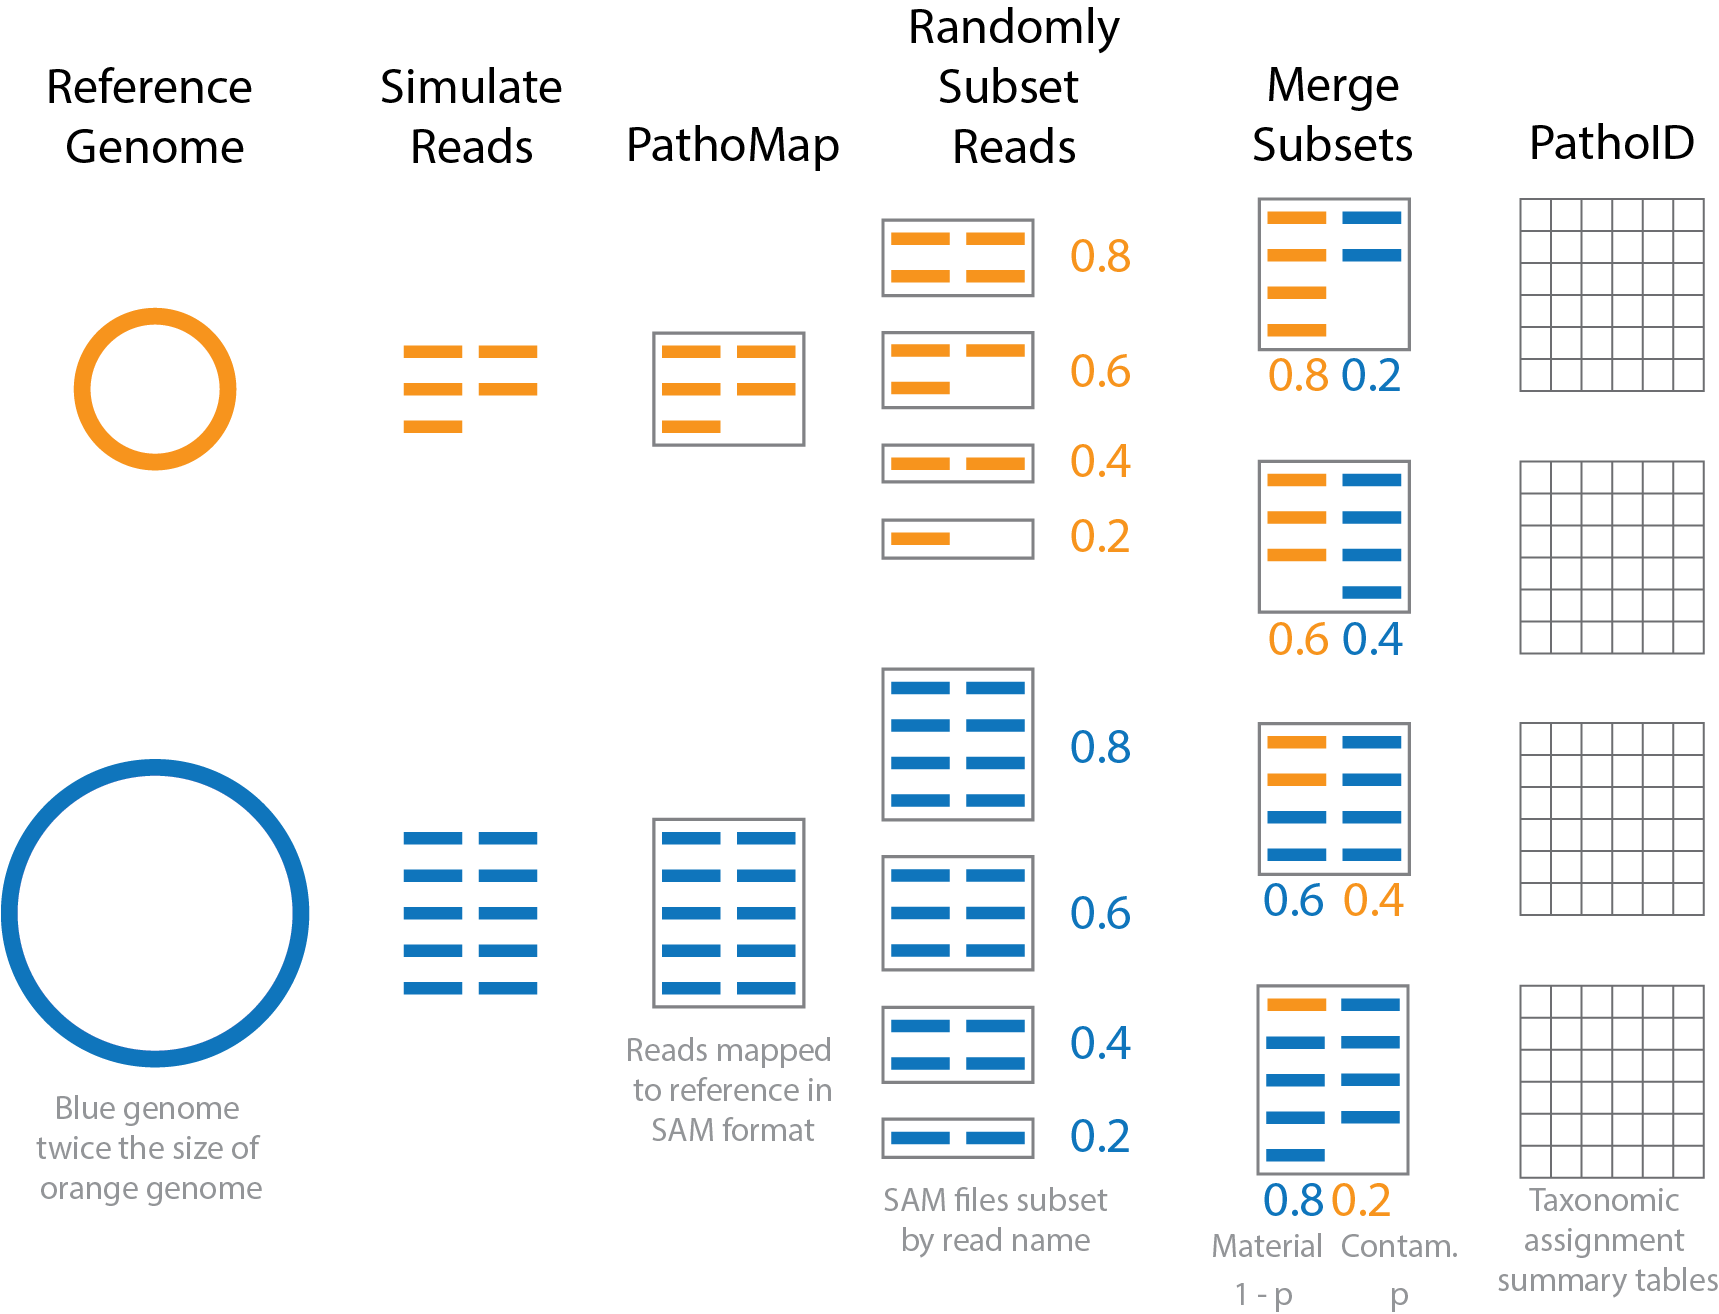
\includegraphics[width=\maxwidth]{figure/contam_simulation} \caption[Diagram of simulated contaminant dataset workflow for two individual genomes]{Diagram of simulated contaminant dataset workflow for two individual genomes. Contaminant proportions (p) of 0.2 and 0.4 are used for demonstration purposes. The reads were initially simulated from individual genomes. The blue genome is twice the size of the orange genome, and twice as many reads are simulated for the blue genome compared to the orange in order to obtain the same coverage. The simulated reads were aligned to the reference database using PathoMap. The resulting alignment file, in SAM file format, was randomly subset based on the desired proportions. Complementary subsets of SAM files (e.g. 0.8 material and 0.2 contaminant) from the two genomes were merged to create individual simulated contaminant datasets.  Due to the different sized genomes, the simulated contaminant datasets have different numbers of reads. Taxonomic assignment summary tables were generated from simulated contaminant datasets using PathoID.}\label{fig:contam_simulation}
\end{figure}


\end{knitrout}


Simulated contaminated datasets were used to evaluate how contaminant detection varied by material and contaminant genome over a range of contaminant concentrations.
Representative genomes for 8 of the 10 genera were used to generate the simulated contaminant datasets (Table \ref{tab:contam_table}, Supplemental Table 2).
An \textit{Escherichia coli} strain was selected as a representative of both \textit{Escherichia} and \textit{Shigella}, as the genus \textit{Shigella} and species \textit{Escherichia coli} are not phylogenetically resolved \citep{lan2002escherichia}. 
No representative genome for \textit{Listeria} was included in this part of the study. 
For each pairwise combination of representative genomes, the simulated contaminant dataset was comprised of a randomly selected subset of reads from the material and contaminant (Fig. \ref{fig:contam_simulation}).
The simulated datasets were randomly subsampled at defined proportions, with $p$ representing the proportion of reads from the contaminant, and $1-p$ the proportion of reads from the material dataset.
A range of contaminant proportions at 10-fold increments was simulated with $p$ ranging from $10^{-1}$ to $10^{-8}$, resulting in 512 simulated contaminant datasets.
This approach simulates the proportion of cells in a contaminated material and not the amount of DNA, assuming unbiased DNA extraction.
Organisms with larger genomes therefore have more simulated reads.


To generate the simulated contaminant datasets, single organism simulated datasets were first generated for the 8 representative genomes using the same methods as baseline assessment (Fig. \ref{fig:contam_simulation}).
The resulting simulated sequencing data was first processed using the PathoQC and PathoMap steps in the PathoScope pipeline.
The output from the PathoMap step (SAM file, sequence alignment file \url{https://samtools.github.io/hts-specs/SAMv1.pdf}) for the material and contaminant datasets were subsampled as described above then combined.
The resulting SAM file was processed by PathoID, the third step in the PathoScope pipeline.
Subsampling the SAM files instead of the simulated sequence files greatly reduces the computational cost of the analysis, as the simulated reads were only processed once by the first two steps in the PathoScope pipeline rather than for every simulated contaminant dataset. 
For simulated datasets with contaminant proportions greater than $10^{-5}$, the quantitative accuracy of the contaminant detection method was assessed by comparing the defined contaminant proportion (true proportion) to the PathoScope contaminant proportion (estimated proportion). 
Pearson's correlation coefficient was used to evaluate agreement between the true and estimated proportions. 
The error rate, $(estimated-true)/true$, was compared across material and contaminant combinations.

\subsection*{Bioinformatics Pipeline}

To facilitate repeatability and transparency, a Docker (\url{www.docker.com}) container is available
with pre-installed pipeline dependencies (\url{www.registry.hub.docker.com/u/natedolson/docker-pathoscope/}).
The scripts used to run the simulations are available at \url{https://github.com/nate-d-olson/genomic_purity}.
Additionally, seed numbers for the random number generator were randomly assigned and recorded for each dataset so the simulated datasets used in the study could be regenerated.
PathoScope results were processed and analyzed using the statistical programming language R \citep{R}, and intermediate analysis and data summaries were organized using ProjectTemplate \citep{ProjectTemplate} and archived in a GitHub repository (\url{https://github.com/nate-d-olson/genomic_purity_analysis}) along with the source files for this manuscript. 


\section*{Results}

\subsection*{Baseline Assessment Using Individual Genomes}

First, we assessed the baseline performance of the proposed contaminant detection method. 
We applied our method to simulated sequencing data from individual genomes. 
All reads assigned to a different taxa than the genome the reads were simulated from were defined as false positive contaminants. 
(This assumes the genome sequence is contaminant free.) 
Our analysis included taxonomic classification results for simulated sequencing data  from 406 genomes, representing 10 different genera (Table \ref{tab:single_org}, Supplemental Table 1).
The method was evaluated using the estimated proportion of species level matches.
The estimated match proportion is the sum of the Final Guess values, proportions reported by PathoScope for a taxa, for all correct species level matches.
For 301 of the 406 genomes, PathoScope estimated that greater than 99\% of the material was the expected species (Fig. \ref{fig:species_prop}).
Of the remaining 105 genomes, the estimated proportion identified as the correct species varied by material genus.
All of the \textit{Shigella} genomes and only 44 of the 49 \textit{Staphylococcus} genomes had estimated proportions for the correct species less than than 0.9.
87 of those 105 genomes come from \textit{Shigella}, \textit{Staphylococcus}, or \textit{Escherichia}.
Excluding \textit{Shigella}, \textit{Escherichia}, and \textit{Staphylococcus}, the median estimated proportion matching at the species level or higher is  0.9996.
We characterized false positive contaminants detected in genomes from the genera \textit{Shigella}, \textit{Escherichia}, and \textit{Staphylococcus}, as well as genomes of other species with match proportions less than 0.9.
Two types of false positive contaminants were identified: (1) contaminants that were genomically indistinguishable from the material and (2) contaminants due to errors in the reference database.

% latex table generated in R 3.3.3 by xtable 1.8-2 package
% Fri Mar 31 10:59:20 2017
\begin{table}[ht]
\centering
\begin{tabular}{lrl}
  \hline
Genus & N & Genome Size (Mb) \\ 
  \hline
\textit{Bacillus} &  76 & 5.05 (3.07-7.59) \\ 
  \textit{Clostridium} &  32 & 4.02 (2.55-6.67) \\ 
  \textit{Escherichia} &  62 & 5.11 (3.98-5.86) \\ 
  \textit{Francisella} &  18 & 1.89 (1.85-2.05) \\ 
  \textit{Listeria} &  39 & 2.97 (2.78-3.11) \\ 
  \textit{Pseudomonas} &  57 & 6.18 (4.17-7.01) \\ 
  \textit{Salmonella} &  44 & 4.88 (4.46-5.27) \\ 
  \textit{Shigella} &  10 & 4.74 (4.48-5.22) \\ 
  \textit{Staphylococcus} &  49 & 2.82 (2.69-3.08) \\ 
  \textit{Yersinia} &  19 & 4.73 (4.62-4.94) \\ 
   \hline
\end{tabular}
\caption{Breakdown of the number of genomes by genus used to generate single genome simulated datasets. N indicates the number of genomes (406 total), and Genome Size is presented as the median and range (minimum to maximum).} 
\label{tab:single_org}
\end{table}


\begin{knitrout}
\definecolor{shadecolor}{rgb}{0.969, 0.969, 0.969}\color{fgcolor}\begin{figure}
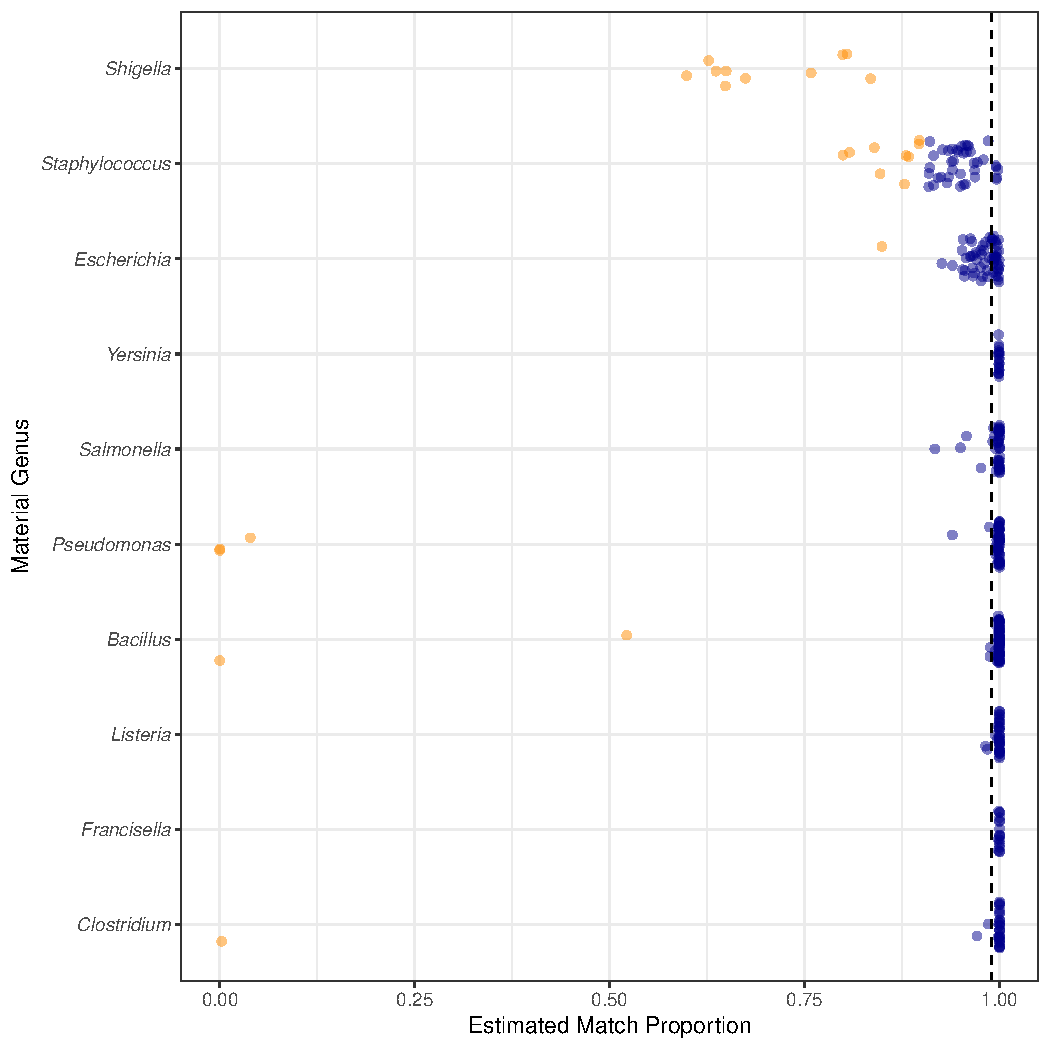
\includegraphics[width=\maxwidth]{figure/species_prop-1} \caption[Species level or higher estimated match proportion varies by material genus]{Species level or higher estimated match proportion varies by material genus. The estimated match proportion is the total proportion of the material with correct taxonomic assignments to the genome species, subspecies, strain, or isolate level. The Estimated Match Proportions shown are the Final Guess values in the PathoScope results table. Each point is calculated for a genome from a different isolate within the genus. The vertical dashed line indicates the 0.99 estimated match proportion. Orange points are genomes with species level estimated match proportions less than 0.90 and blue points greater than or equal to 0.90.}\label{fig:species_prop}
\end{figure}


\end{knitrout}

Two genomes can be genomically indistinguishable if the majority of the two genome sequences are highly similar.
Phylogenetically closely related organisms are expected to have large genomic regions with high levels of similarity.
Phylogenetic similarity is at least partially responsible for the low species level estimated match proportion for  \textit{Shigella} and \textit{Escherichia}, as \textit{Shigella} is not phylogenetically distinct from \textit{E. coli} \citep{lan2002escherichia}.
When including matches to \textit{E. coli} as species level matches, the median estimated match proportions for \textit{Shigella} genomes increases from 0.66 to 0.92.
Another example of false positives at the species level due to phylogenetic similarity was low match percentage for \textit{Clostridium autoethanogenum} strain DSM10061, where \textit{Clostridium ljungdahlii} strain DSM13528 was assigned the top proportion of reads (0.998) instead of \textit{C. autoenthanogenum}.
False positive contaminants due to phylogenetic similarity are not limited to a closely related species or genus.
\textit{Escherichia coli} strain UMNK88 low match proportions were due to two bacteria in the same family as \textit{E. coli}
(Enterobacteriaceae): \textit{Providencia stuartii} and \textit{Salmonella enterica} subsp. \textit{enterica} serovar Heidelberg, which had estimated proportions of 0.11 and 0.03, respectively.
False positives were also due to shared genetic material between bacteria and their phage.
Phage were identified as false positive contaminants at varying proportions for genomes from all genera investigated, excluding \textit{Francisella} (Fig. \ref{fig:phage_prop}).
The low proportions of species level matches for \textit{E. coli} and \textit{Staphylococcus} are partly due to relatively higher proportions of matches to phage, compared to the other genera investigated.
Based on phage names, all of the false positive phage contaminants were specific to the taxonomy of the material genome.

\begin{knitrout}
\definecolor{shadecolor}{rgb}{0.969, 0.969, 0.969}\color{fgcolor}\begin{figure}
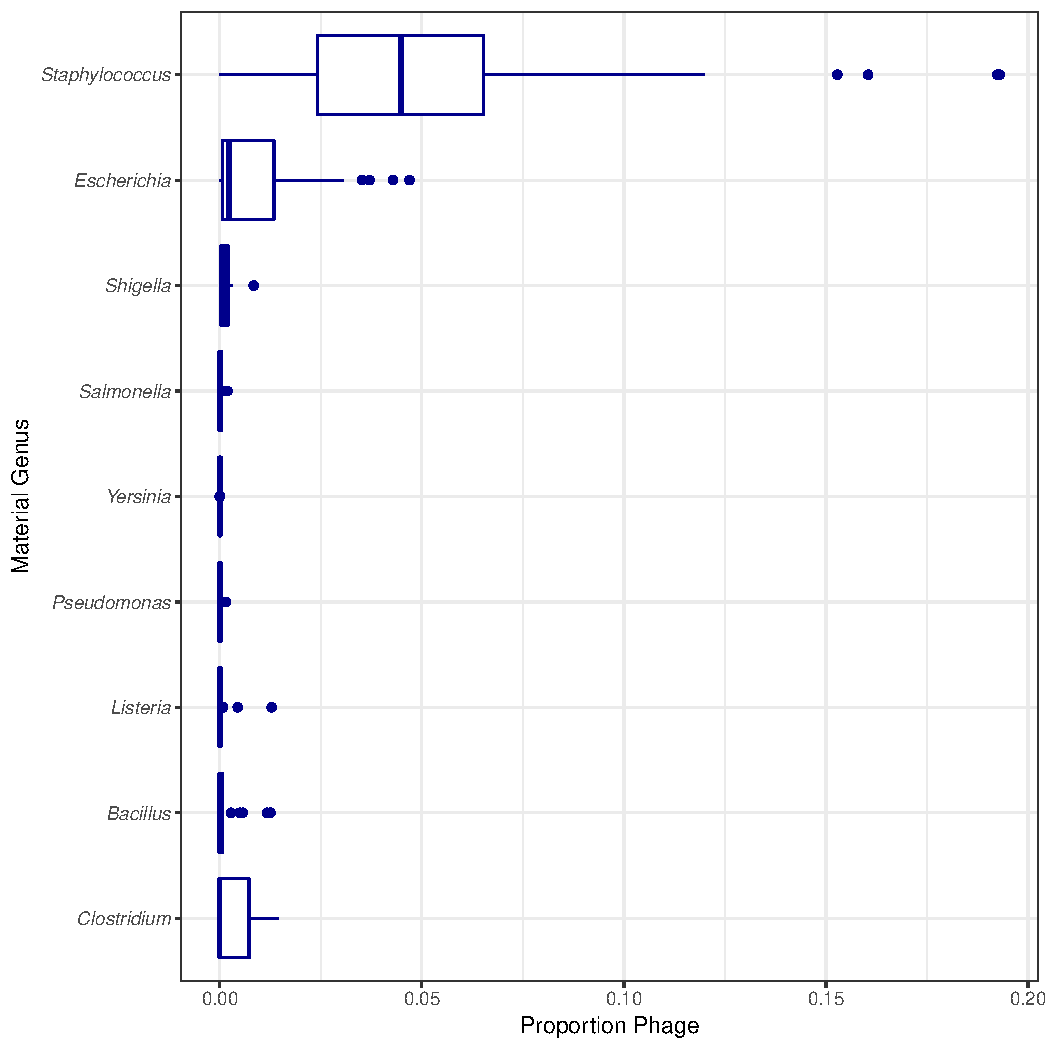
\includegraphics[width=\maxwidth]{figure/phage_prop-1} \caption[Estimated proportion of phage in the simulated single genome datasets by genera]{Estimated proportion of phage in the simulated single genome datasets by genera. Final Guess values reported by PathoScope used to calculate estimated proportions. No phage were reported by PathoScope for any \textit{Francisella} genomes.}\label{fig:phage_prop}
\end{figure}


\end{knitrout}


False positive contaminants were also due to potential errors in the database such as unclassified or misclassified sequences and the presence of genome assemblies in the database containing sequence data from organismal or reagent contaminants.
Low estimated match proportions can also be due to the database containing unclassified sequence data for organisms with genomic regions that are highly similar to regions of the material genome.
For example, the low estimated match proportion for \textit{Pseudomonas} strain FGI182 was due to matches to unclassified bacteria, bacterium 142412, and unclassified \textit{Pseudomonas} species, \textit{Pseudomonas} sp. HF-1.
The low estimated match proportion proportion of species level matches for \textit{Pseudomonas} strain TKP was also due to potentially misclassified sequences (\textit{Thioalkalivibrio sulfidophilus} strain HL-EbGr7, estimated match proportion 0.0648).
\textit{Bacillus subtilis} BEST7613 genome had low species level estimated match proportion due to \textit{Synechocystis} sp. PCC 6803 substr. PCC-P being estimated as comprising 47\% of the material.
\textit{Synechocystis} is in a different phylum compared to \textit{Bacillus} (cyanobacteria versus firmicutes) and is a false positive due to a misclassification.
The \textit{Bacillus subtilis} BEST7613 genome in the database is a synthetic chimeric genome constructed from \textit{Bacillus subtilis} BEST7613 and \textit{Synechocystis} sp. PCC 6803 substr. PCC-P not \textit{Bacillus subtilis} BEST7613 \citep{watanabe2012complete}. 
The \textit{Bacillus subtilis} BEST7613 genome assembly (GenBank Accession GCA\_000328745.1) was flagged by the databases curators as an anomalous assembly and removed from the RefSeq database.  
The genome sequences used to populate the reference database can contain contaminants themselves \citep{parks2015checkm}.
These database contaminants are responsible for additional false positive contaminants.
The species level estimated match proportion for \textit{Pseudomonas} strain TKP was partially due to contaminated genome sequences in the database (wheat - \textit{Triticum aestivum} estimated match proportion 0.087).
The eukaryotic false positive contaminants are likely due to contaminants in the eukaryotic DNA extract or reagents used to generate the sequencing data for the assembly \citep{parks2015checkm}.

\subsection*{Contaminant Detection Assessment}

% latex table generated in R 3.3.3 by xtable 1.8-2 package
% Fri Mar 31 10:59:21 2017
\begin{table}[ht]
\centering
\scalebox{0.85}{
\begin{tabular}{lrrr}
  \hline
Representative Strain & Match Proportion & Aligned Reads & Mb \\ 
  \hline
\textit{Bacillus anthracis} str. Ames & 1.00 & 227270 & 5.23 \\ 
  \textit{Clostridium botulinum} A str. Hall & 1.00 & 163500 & 3.76 \\ 
  \textit{Escherichia coli} O157:H7 str. EC4115 & 0.98 & 247990 & 5.70 \\ 
  \textit{Francisella tularensis} subsp. \textit{tularensis} SCHU S4 & 1.00 & 82290 & 1.89 \\ 
  \textit{Pseudomonas aeruginosa} PAO1 & 1.00 & 272360 & 6.26 \\ 
  \textit{Salmonella enterica} subsp. \textit{enterica} serovar Typhimurium str. D23580 & 1.00 & 212140 & 4.88 \\ 
  \textit{Staphylococcus aureus} subsp. \textit{aureus} ED133 & 0.98 & 123150 & 2.83 \\ 
  \textit{Yersinia pestis} CO92 & 1.00 & 209970 & 4.83 \\ 
   \hline
\end{tabular}
}
\caption{Representative strains used in simulated contaminant datasets, based on available type strains. Match proportion indicates the estimated proportion of the material assigned to the correct species by PathoScope. Aligned Reads is the number of simulated reads aligned to the database by PathoMap. DNA size is the total size of the genome, chromosome and plasmids in Mb.} 
\label{tab:contam_table}
\end{table}



Finally, contaminant detection was assessed by combining subsets of simulated data from two organisms at defined proportions,
with the larger proportion representing the microbial material and smaller proportion the contaminant (Fig. \ref{fig:contam_simulation}).
We simulated contaminant datasets as pairwise combinations of representative genomes from 8 of the genera used in the baseline assessment section of the study (Table \ref{tab:contam_table}).
All of the genomes selected have a species level estimated match proportion greater than 0.98 (Table \ref{tab:contam_table}).

The minimum contaminant proportion detected was $10^{-3}$ and  $10^{-4}$ for most pairwise comparisons with a few exceptions (Fig. \ref{fig:contam_fig}).
When \textit{Y. pestis} was the simulated contaminant, the minimum detected proportion was 0.1 for all material strains.
For all simulated datasets where \textit{F. tularensis} was the contaminant, the contaminant was not detected. 
It is unclear why \textit{Y. pestis} was only detected at a higher proportion relative to the other datasets, $10^{-1}$ versus $10^{-3}$, and \textit{F. tularensis} was not detected at all.
One possible reason for the lower contaminant detection for these two organisms is that there are fewer genomes in the database for these two genera.
Additionally, the \textit{F. tularensis} dataset is much smaller relative to the other genera, less than 90,000 reads.
Therefore, with fewer reads in the dataset and genomes in the database, the probability that the randomly selected subset of reads spiked into the simulated material dataset contains reads allowing for contaminant detection is lower. 
A few contaminants were detected at proportions as low as $10^{-8}$, such as when \textit{Yersinia} contaminated with \textit{E. coli} or \textit{S. enterica}.
However, contaminants detected at lower proportions were due to reads simulated from the material genome incorrectly assigned to the contaminant.
The simulated contaminant-free \textit{Y. pestis} material dataset had false positive reads assigned to two of the contaminants resulting in artificially low contaminant detection proportions for \textit{Salmonella enterica} subsp. {enterica} serovar Typhi str. CT18 and \textit{Escherichia coli} O104:H4 str. 2011C-3493 with estimated proportions of \ensuremath{1.76\times 10^{-5}}and \ensuremath{3.77\times 10^{-8}}, respectively. 
The simulated dataset coverage accounts for the observed minimum dectected contaminant proportion.
As the individual datasets were simulated at 20X coverage, \textless 300,000 reads were simulated for each dataset, and on average \textless 3 reads were spiked into the material datasets for simulated contaminant proportions $\leq$ $10^{-5}$ (Fig. \ref{fig:contam_fig}).

\begin{knitrout}
\definecolor{shadecolor}{rgb}{0.969, 0.969, 0.969}\color{fgcolor}\begin{figure}
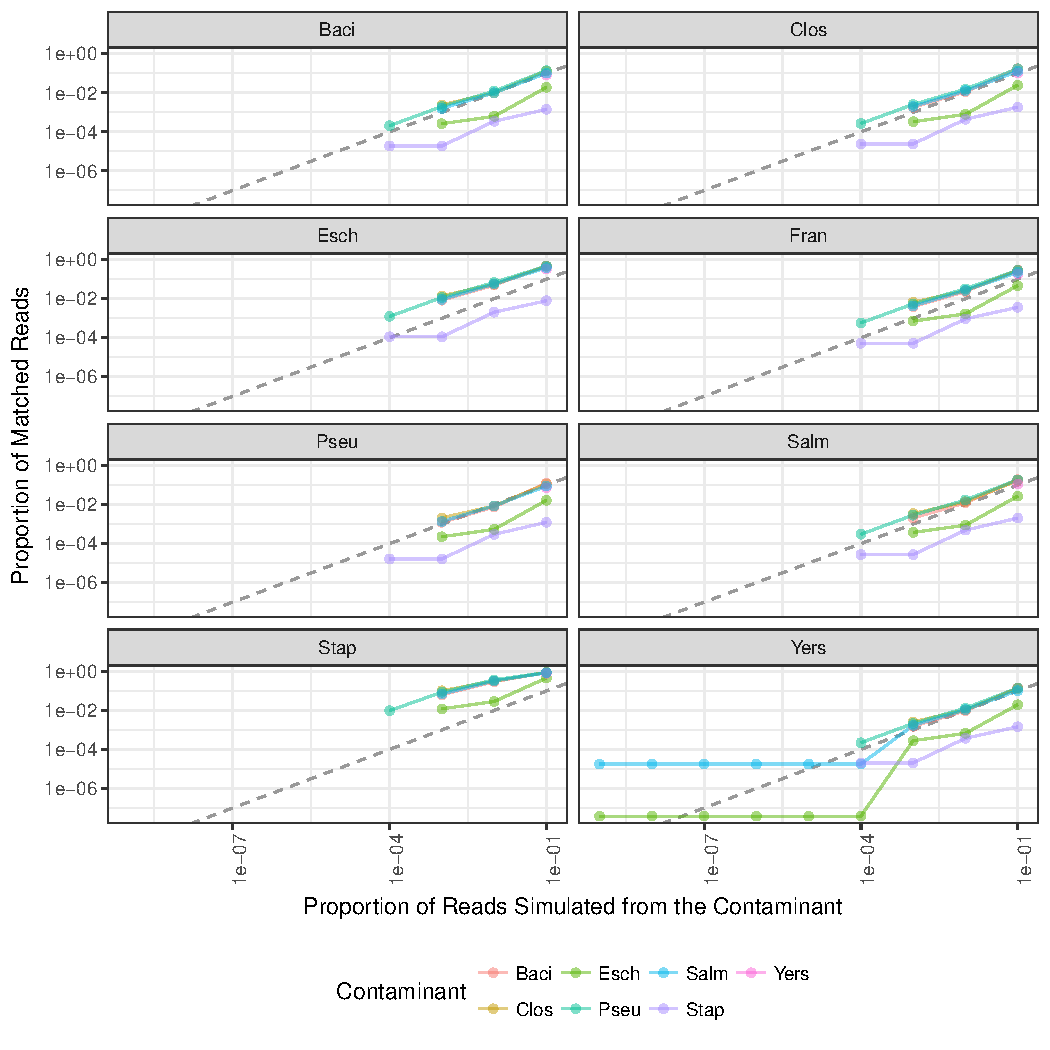
\includegraphics[width=\maxwidth]{figure/contam_fig-1} \caption[The relationship between the proportion of reads matching the contaminant species and the proportion of simulated contaminant reads]{The relationship between the proportion of reads matching the contaminant species and the proportion of simulated contaminant reads. Plots are split by the material species with line and point color indicating contaminant species. Dashed line indicates the expected 1:1 correlation between the proportion of reads matching the expected contaminant and the proportion of reads simulated from the contaminant. The contaminant proportion was underestimated for points below the dashed line and overestimated for points above the dashed line.}\label{fig:contam_fig}
\end{figure}


\end{knitrout}


\begin{knitrout}
\definecolor{shadecolor}{rgb}{0.969, 0.969, 0.969}\color{fgcolor}\begin{figure}
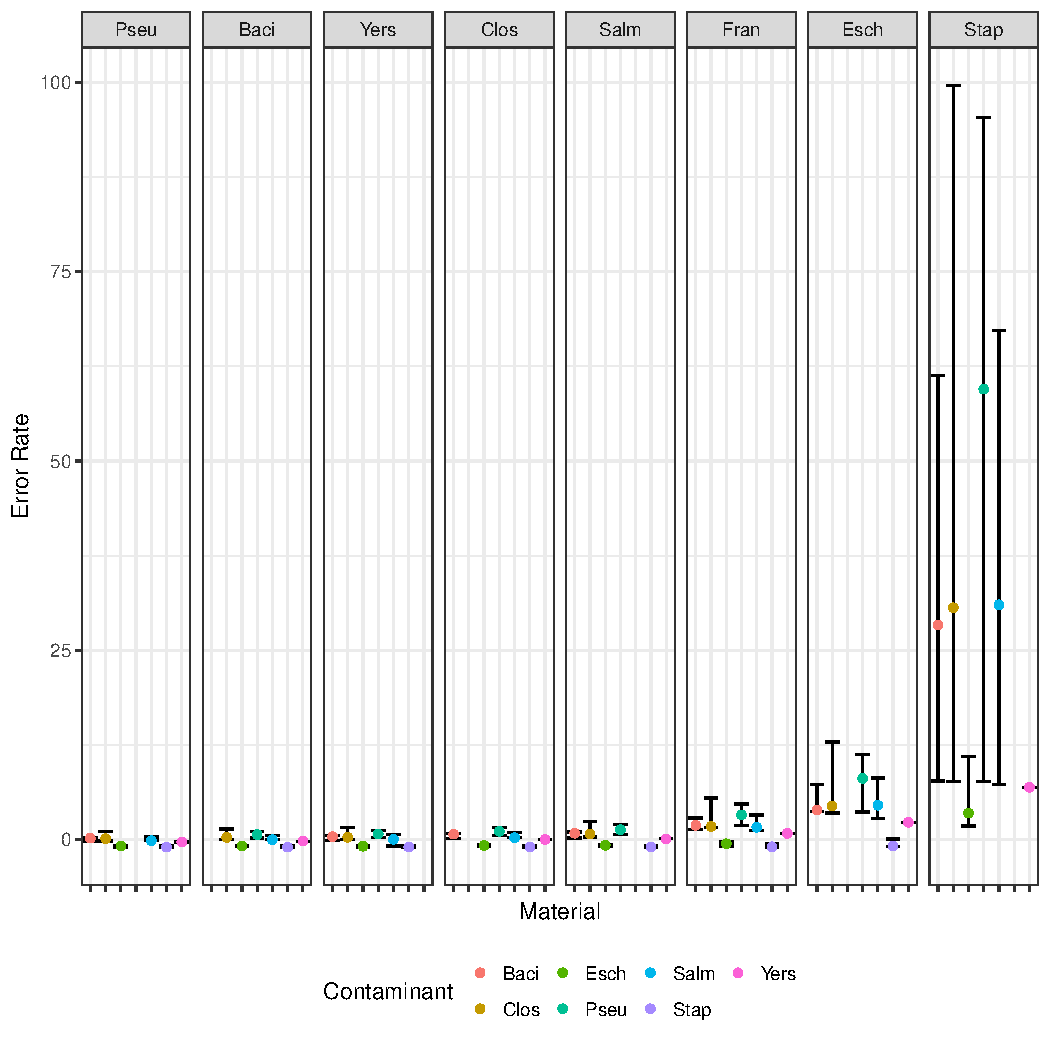
\includegraphics[width=\maxwidth]{figure/contam_resid-1} \caption[Error rate, $(estimated - true)/true$, for pairwise combinations of material and contaminant]{Error rate, $(estimated - true)/true$, for pairwise combinations of material and contaminant. Points and error bars represent the median and range (minimum - maximum) error rate for each material and contaminant combination.}\label{fig:contam_resid}
\end{figure}


\end{knitrout}

In addition to the minimum detected contaminant proportion, we also evaluated the quantitative accuracy of the contaminant detection method.
Pearson's correlation coefficient was used to determine the correlation between the estimated contaminant and true contaminant proportions for simulated contaminant proportions greater than $10^{-6}$.
The estimated and true proportions were strongly correlated for all pairwise comparisons, with an overall median and 95\% confidence interval of 0.99945 (0.96945 - 1) (Fig. \ref{fig:contam_fig}).
Eight of the pairwise comparisons have correlation coefficients below 0.99, all of which have \textit{S. aureus} as either the contaminant or the material.
Two coefficients were below 0.98: \textit{S. aureus} contaminated with \textit{P. aeruginosa} and \textit{S. enterica}, 0.952 and 0.969 respectively.
The total error rate was used to assess the accuracy of the PathoScope contaminant proportion estimates (Fig. \ref{fig:contam_resid}).
The material genome strongly influenced the total error rate with \textit{E. coli} and \textit{S. aureus} having consistently higher total error rates compared to the other genomes, indicating a reduced accuracy for the two species.


\section*{Discussion}

The potential for using whole genome sequence data and taxonomic sequence classification algorithms to detect contaminant DNA in microbial materials was evaluated.
The method requires no \textit{a priori} information about the contaminant and can identify common as well as unexpected contaminants.
Additionally, as whole genome sequencing can be performed on genomic DNA and cell cultures (after DNA extraction), the method is appropriate for both types of microbial materials.
A baseline assessment of the contaminant detection method using simulated sequencing data from individual genomes was performed to identify common types of classification errors that would result in false positive contaminants.
The false positive contaminants were split into two categories (1) those due to an inability of the method to differentiate the material genome from the contaminant genome, and (2) errors in the reference database.
Contaminant detection performance was characterized for different material, contaminants, and contamination level.
Overall the method was able to identify contaminant proportions at $10^{-3}$ for most contaminant-material combinations. 
This level of detection is dependent on not just the classification method but also the simulated coverage. 
Therefore a lower detection proportion is expected for increased coverage. 
A contaminant proportion of $10^{-3}$ is equivalent to 1 contaminant cell per 1,000 cells in a microbial material, or 1,000 contaminant cells in 1 mL of a $10^{6}$ cells/mL culture.
The estimated contaminant proportion accuracy for the simulated contaminated material varied by contaminant and material strain.

There are three basic steps to using this method to detect contaminants in a microbial material. 
Baseline assessment is the first step. 
For a baseline assessment, reads are simulated from the reference genome of the organism of interest and processed using a taxonomic classification algorithm. 
Performing a baseline assessment allows one to identify the false positive contaminants you can expect to observe due to limitations in the method. 
Simulating data with realistic error profiles, read length, and fragment distribution is likely to yield results more representative of what one would expect from real sequencing data.
Next, sequencing data generated from the microbial material is processed using the same taxonomic classification algorithm as used in the baseline assessment. 
The last step is a critical evaluation of results for potential false positives. 
For all settings including research, clinical, regulatory, and attribution, the contaminant detection method should be validated for the intended application.
Appropriate validation approaches may include experiments with simulated contaminants like those performed as part of this study and sequencing genomic DNA or cells spiked with varying contaminant concentrations.

It is important to evaluate the results in the context of the intended application.
Quantitative accuracy in contaminant proportions is important for applications where acceptable contaminant proportion thresholds are established.
For example, a microbial material with a contaminant proportion of $10^{-5}$ may be acceptable for use in an assay where the contaminant adversely impacts an assay when present in proportions greater than $10^{-4}$.
Quantitative accuracy is also relevant when performing a general characterization of the microbial material.
General contaminant characterization is appropriate for reference materials with more than one use case such as the NIST microbial genomic reference materials (NIST RM8375) \citep{olson2016pepr}.
Similar to the false positive contaminant baseline assessment,
simulated data can be used to evaluate the minimal detectable contaminant proportion for specific organisms using different taxonomic assignment algorithms and databases.

A primary limitation of the proposed method is the observed false positive contaminants identified in the baseline assessment. 
The reference database and taxonomic assignment algorithm are likely to impact the number and types of false positives. 
There are three primary types of taxonomic read classification algorithms: sequence similarity search, sequence composition methods, and phylogenetic methods \citep{Bazinet2012}. 
The algorithm used in this study, PathoScope, is a type of sequence similarity search algorithm. 
Evaluating different types of algorithms using simulated data for the material genome of interest, similar to what was done in the baseline assessment part of this study, would help determine the optimal classification algorithm for a specific microbial material. 
Furthermore, recent advances in taxonomic classification algorithms have led to the development of faster methods, including Kaiju, a sequence composition type method, and Centrifuge, a sequence similarity search type method \citep{menzel2016fast,Kim2016-ir}. 
Application of these new methods would lower the computational cost of the baseline assessment. 

A number of the observed false positives were due to errors in the database and inability of the taxonomic classification algorithm to correctly identify the source of the sequence when it matches multiple organisms in the database. 
Removing sequences from the database for irrelevant contaminants, such as phage, plasmids, vectors, and multicellular eukaryotes, would reduce the proportion of false positives.
By excluding irrelevant contaminants from the database, sequencing reads aligning to these irrelevant sequences would no longer result in false positive contaminants.
Methods for excluding sequence data from a reference database are dependent on the classification algorithm used.
For example, user-specified sequence data could be removed from the reference database by PathoScope using the PathoDB function.
Caution should be used when removing sequences from a reference database.
For example, vector sequences from contaminants in sequencing reagents, if excluded from the database may be incorrectly classified as an organismal contaminant.
Similarly, using a curated database free of misclassified and unclassified sequence data would further reduce the proportion of false positive contaminants \citep{tennessen2015prodege}.
For example, the \textit{Bacillus subtilis}-\textit{Synechocystis} chimeric genome appeared to have a high false positive contaminant rate in the baseline assessment part of this study due to the genome being incorrectly classified as \textit{Bacillus subtilis} and not a chimeric genome.


\section*{Conclusions}
Identification and characterization of low abundance contaminants in a non-targeted manner is critical for a material used in high sensitivity assays such as PCR.
With the continual decline in the cost of sequencing and advances in sequence analysis methods, whole genome sequencing combined with taxonomic assignment algorithms provides a viable alternative to commonly used organismal contaminant detection methods such as culturing, microscopy, and PCR.
The method presented here is suitable for detecting organismal contaminants in both genomic DNA and whole cell microbial materials, with the only \textit{a priori} assumption that the contaminant is in the reference database. 
The false positive contaminant detection is a primary limitation of the proposed method. 
As false positive contaminants are database and taxonomic assignment algorithm dependent, additional work is needed to improve database curation and data authentication efforts as well as characterize taxonomic assignment algorithm performance.

\newpage

\section*{Acknowledgments}

The authors would like to thank Dr. Steven Lund for his assistance in developing the study.
The Department of Homeland Security (DHS) Science and Technology Directorate supported this work under the Interagency Agreement HSHQPM-15-T-00019 with the NIST.
Opinions expressed in this paper are the authors’ and do not necessarily reflect the policies and views of DHS,  NIST, or affiliated venues.
Certain commercial equipment, instruments, or materials are identified in this paper in order to specify the experimental procedure adequately.
Such identification is not intended to imply recommendations or endorsement by NIST,
nor is it intended to imply that the materials or equipment identified are necessarily the best available for the purpose.
Official contribution of NIST; not subject to copyrights in USA.

\bibliography{genomic_purity}

\end{document}

%% Genome Comparison Text
%% Genbank - VISTA alignment available for 30 days from 11/16/2016
% \textit{Clostridium autoethanogenum} strain DSM10061 https://www.ncbi.nlm.nih.gov/nuccore/NC_022592.1
% \textit{Clostridium ljungdahlii} strain DSM13528 https://www.ncbi.nlm.nih.gov/nuccore/NC_014328.1
% Large number of highly similar regions based on VISTA whole genome alignment
% http://pipeline.lbl.gov/tbrowser/tbrowser/?run=42512-C9RZqeQ4

% \textit{Escherichia coli} strain UMNK88 https://www.ncbi.nlm.nih.gov/nuccore/NC_017641.1
% \textit{Providencia stuartii} https://www.ncbi.nlm.nih.gov/nuccore/NC_017731.1
% VIST whole genome alignment http://pipeline.lbl.gov/tbrowser/tbrowser/?run=42979-2ayB76PW

% \textit{Escherichia coli} strain UMNK88 https://www.ncbi.nlm.nih.gov/nuccore/NC_017641.1
% \textit{Salmonella enterica} subsp. \textit{enterica} serovar Heidelberg https://www.ncbi.nlm.nih.gov/assembly/GCF_001690135.1 Only compared chromosome
% VISTA whole genome alignment http://pipeline.lbl.gov/tbrowser/tbrowser/?run=42980-poO1BFgN
